\chapter{Modelo de Capa Delgada}
\label{chap:hipersonica}

Un ejemplo más realista para la forma de los choques de proa proviene de modelos hidrodinámicos en estado estacionario de la interacción de flujos hipersónicos en el límite de capa delgada. Ejemplos clásicos son la interacción entre dos vientos de \citet{Canto:1996} (\CRW {}de aquí en adelante)y la interacción entre un viento con una corriente plano--paralela \citep{Wilkin:1996}. 
%El problema de interacción de dos vientos es de gran interés en astrofísica, y ha sido estudiado en múltiples ocasiones, principalmente mediante simulaciones hidrodinámicas. Sin embargo, cuando se toman en cuenta diversos factores, incluídos conservación de masa, momento y momento angular, el problema puede resolverse de manera algebraica.
\section{Cantidades conservadas en un flujo hipersónico de capa delgada}

Consideramos dos flujos hipersónicos, no acelerados que forman una capa estacionaria delgada formada por dos choques radiativos separados por una discontinuidad de contacto. El sistema tiene geometría cilíndrica y los vientos no tienen velocidad azimutal. Bajo estos términos, describimos la posición de la capa delgada como $R(\theta)$, donde $R$ es el radio de la capa medido a partir de la posición del origen del viento con menor momento y $\theta$ es el ángulo polar. Asumimos que el gas chocado está bien mezclado, esto implica que  tiene una sola velocidad pos--choque dada por:

\begin{align}
  \vec{v} = v_r \hat{r} + v_z \hat{z}
\end{align}

Donde el eje de simetría del sistema es paralelo a $\hat{z}$, y $\hat{r}$ es el radio cilíndrico. Definimos $\dot{M}(\theta)$, $\vec{\dot{\Pi}}(\theta)$ y $\dot{J}(\theta)$ como la tasa de pérdida de masa, la tasa de momento y la tasa de momento angular, respectivamente, de la capa delgada integradas desde $\theta=0$ hasta $\theta$. Éstas se calculan de la siguiente manera:

\begin{align}
  \vec{\dot{\Pi}}(\theta) &= \dot{\Pi}_r(\theta) \hat{r} + \dot{\Pi}_z(\theta) \hat{z} = \dot{M}\left(v_r \hat{r} + v_z\hat{z}\right) \label{eq:dot-pi}\\
  \vec{\dot{J}}(\theta) &= \vec{R}(\theta) \times \vec{\dot{\Pi}}(\theta)  \\
  \dot{M}(\theta) &= \dot{M}_w(\theta) + \dot{M}_{w1} \label{eq:dot-M}
\end{align}
Donde $\vec{R}(\theta)\equiv R(\theta)\sin\theta~\hat{r} + R(\theta)\cos\theta~\hat{z}$. Resolviendo el producto cruz y tomando su magnitud encontramos que:
\begin{align}
  \dot{J}(\theta) &= \dot{M}(\theta)R(\theta)v_\theta \label{eq:dot-J}\\
  \mathrm{donde:~} & v_\theta = v_r\cos\theta - v_z\sin\theta \label{eq:v-theta}
\end{align}

Por otro lado, al asumir estado estacionario, necesitamos que la tasa de pérdida de masa, la tasa de momento y la tasa de momento angular de la capa delgada sean iguales a aquellas inyectadas por los dos vientos. Entonces definimos estas cantidades como $\dot{M}_w$, $\dot{\Pi}_{wr}$, $\dot{\Pi}_{wz}$ y $\dot{J}_{w}$ para el viento con menor momento, y para el otro viento se utiliza la misma notación solo que utilizando el subíndice ``w1''. De esta forma tenemos que:
\begin{align}
  \dot{\Pi}_r(\theta)\hat{r} + \dot{\Pi}_z(\theta)\hat{z} &= \left[\dot{\Pi}_{wr}(\theta)+ \dot{\Pi}_{wr1}(\theta)\right]\hat{r} + \left[\dot{\Pi}_{wz}(\theta)+ \dot{\Pi}_{wz1}(\theta)\right]\hat{z} \label{eq:Pi-2} \\
  \dot{J} &=\dot{J}_w(\theta) + \dot{J}_{w1}(\theta) \label{eq:J-2}\\
  \dot{M}(\theta) &= \dot{M}_w(\theta) + \dot{M}_{w1}(\theta) \label{eq:M-2}
\end{align}

Combinando las ecuaciones (\ref{eq:dot-pi}), (\ref{eq:dot-J}), (\ref{eq:dot-M}), (\ref{eq:Pi-2}), (\ref{eq:J-2}) y (\ref{eq:M-2}) encontramos que:

\begin{align}
  \dot{M}(\theta)\left[v_r \hat{r} + v_z\hat{z}\right] &= \left(\dot{\Pi}_{wr}(\theta) + \dot{\Pi}_{wr1}(\theta)\right)\hat{r} +
                                                         \left(\dot{\Pi}_{wz}(\theta) + \dot{\Pi}_{wz1}(\theta)\right)\hat{z} \\
  \dot{M}(\theta)v_\theta R(\theta) &= \dot{J}_w(\theta) + \dot(J)_{w1}(\theta)
\end{align}
Y finalmente combinando con la ecuación (\ref{eq:v-theta}) resolvemos para $R(\theta)$:
\begin{align}
  R(\theta) = \frac{\dot{J}_w(\theta) + \dot(J)_{w1}(\theta)}{\left(\dot{\Pi}_{wr}(\theta) + \dot{\Pi}_{wr1}(\theta)\right)\cos\theta - \left(\dot{\Pi}_{wz}(\theta) + \dot{\Pi}_{wz1}(\theta)\right)\sin\theta} \label{eq:R-wind}
\end{align}



\section{Problema de Interacción de Dos Vientos}
\label{sec:CRW-2-winds}
Aplicamos el formalismo ya mencionado para la interacción de dos vientos radiales. El viento con menor momento se localiza en el origen, y su densidad a radio fijo varía con el ángulo polar como una ley de potencias
(figura \ref{fig:isotropic-aniso}):
\begin{align}
  n(\theta) = n_0\cos^k\theta \label{eq:anisotropic-density}
\end{align}
Donde el índice $k$ indica el grado de anisotropía del viento ``interno''. Cuando $k = 0$ denominamos a los choques resultantes como ``cantoides'', por \citet{Canto:1996}, mientras que en el resto de los casos los denominamos ``Ancantoides''. Un caso particularmente interesantes son el viento para un proplyd \citep{HA:1998}, donde $(k=1/2)$. Por el momento restringimos al viento ``externo'' como isotrópico. El problema se muestra de manera esquemática en la figura \ref{fig:crw-esquema}.

Utilizando la ecuación (\ref{eq:anisotropic-density}) encontramos que la tasa de pérdida de masa está dada por:

\begin{align}
  \dot{M}_w = \int^\theta_0\int^{2\pi}_0\rho_w v_w~d\theta~d\phi =
  \frac{M^0_w}{2\left(k+1\right)}\left(1 - \cos^{k+1}\theta\right) \label{eq:inner-dot-M}
\end{align}
Donde $v_w$ es la velocidad del viento inteno, $\rho_w = n\bar{m}$  es su densidad, $n$ se obtiene de la ecuación (\ref{eq:anisotropic-density}), $M^0_w = 4\pi r^2_0v_w n_0 \bar{m}$ es la tasa de pérdida de masa integrada hasta
$\theta = \pi$ para un viento isotrópico, $\bar{m}$  es la masa promedio de las partículas del viento y $r_0$ es el radio del viento al cual se alcanza la velocidad terminal $v_w$. Para un proplyd consideramos que dicho
radio es el del frente de ionización.

Con esto, obtenemos las tasas de momento y momento angular:
\begin{align}
  \dot{\Pi}_{wz} &= \int^\theta_0 v_w\cos\theta~d\dot{M}_w = \frac{v_w \dot{M}^0_w}{2\left(k+2\right)}\left(1 - \cos^{k+2}\theta\right) \label{eq:Pi-wz} \\
  \dot{\Pi}_{wr} &= \int^\theta_0 v_w\sin\theta~d\dot{M}_w = \frac{1}{2}\dot{M}^0_w v_w I_k(\theta) \\
  \dot{J}_w &= \int^\theta_0 |\vec{R} \times \vec{v}_w|d\dot{M}_w = 0 \label{eq:inner-dot-J}
\end{align}

Donde la integral $I_k(\theta) = \int^\theta_0 \cos^k\theta \sin^2\theta~d\theta$ tiene solución analítica para $k=0$, es una integral elíptica de segundo tipo cuando $k=\frac{1}{2}$ y su solución es aun más compleja para el resto de los
casos. Las tasa de momento angular para el viento interior es cero debido a que éste se mide respecto al origen, donde se localiza la fuente con menor momento. En este punto los vectores de posición y velocidad para un valor de $\theta$
dado son paralelos.

Para el viento exterior consideramos dos casos principales: un viento esférico e isotrópico y un viento plano--paralelo de densidad y velocidad constante.

\subsection{Interacción con un viento esférico isotrópico}
\label{sec:mod-isotropic}
En este caso tomamos como variable independiente al ángulo polar medido a partir de la posición de la fuente del viento externo, denotado por $\theta_1$. De esta forma las tasas de pérdida de masa, momento y momento angular quedan como sigue:

\begin{align}
  \dot{M}_{w1} &= \frac{M^0_{w1}}{2}\left(1 - \cos\theta_1\right)\\
  \dot{\Pi}_{wz1} &= -\frac{v_{w1}\dot{M}^0_{w1}}{4}\sin^2\theta_1\\
  \dot{\Pi}_{wr1} &= \frac{v_{w1}\dot{M}^0_{w1}}{4}\left(\theta_1 - \sin\theta_1\cos\theta_1\right)\\
  \dot{J}_{w1} &= \int^{\theta_1}_0 R(\theta)v_{w1}\sin(\pi-\theta-\theta_1)~d\dot{M}_{w1} \label{eq:J1}
\end{align}

Utilizando la ley de los senos (ver figura \ref{fig:crw-esquema}), la ecuación (\ref{eq:J1}) queda como sigue:

\begin{align}
  \dot{J}_{w1} &= Dv_{w1}\int^{\theta_1}_0 \sin\theta_1~d\dot{M}_{w1} =
                 \frac{v_{w1}\dot{M}^0_{w1}}{4}\left(\theta_1 - \sin\theta_1\cos\theta_1\right) D \label{eq:J1-iso}
\end{align}

Por otro lado, de la figura \ref{fig:crw-esquema}, podemos deducir la siguiente relación geométrica entre $R(\theta)$,
$\theta$ y $\theta_1$:
\begin{align}
  \frac{R(\theta)}{D} &= \frac{\sin\theta_1}{\sin(\theta+\theta_1)} \label{eq:R-geometric}
\end{align}

Combinando las ecuaciones (\ref{eq:R-wind}), (\ref{eq:Pi-wz}) - (\ref{eq:J1-iso}) y (\ref{eq:R-geometric}) obtenemos una ecuación
implícita que nos indica la dependencia de $\theta_1$ con $\theta$:

\begin{align}
  \theta_1\cot\theta_1 -1 = 2\beta I_k(\theta)\cot\theta - \frac{2\beta}{k+2}\left(1 - \cos^{k+2}\theta\right) \label{eq:th1-th} 
\end{align}
Donde $\beta = \frac{\dot{M}^0_w v_w}{\dot{M}^0_{w1}v_{w1}}$ es el cociente del momentos entre los vientos. Este parámetro, junto con el índice de anisotropía $k$ son los que determinan la forma del choque de proa. 

El radio en el ápex, la planitud y la alatud en este caso se muestran a continuación. El procedimiento detallado se puede consultar en el apéndice \ref{app:derivation-radii}:

\begin{align}
  \frac{R_0}{D} &= \frac{\beta^{1/2}}{1+\beta^{1/2}} \\
  \Lambda &= \frac{\left(3\xi\right)^{1/2}\left(1+\beta^{1/2}\right)}
                     {\left(1+\frac{1}{5}\xi\beta\right)^{1/2}\left(1-\xi\beta\right)} \label{eq:CRW-R90}\\
  \Pi &= \left|1 - 2R_{\theta, \theta}\right|^{-1} \label{eq:CRW-Rc}\\
  \mathrm{Donde:~} R_{\theta, \theta} &= \frac{C_{k\beta}}{1+\beta^{1/2}} + \frac{1 + 2\beta^{1/2}}{6} \label{eq:2-order}
\end{align}


\subsection{Interacción de un viento esférico isotrópico con un viento plano--paralelo (Choques Wilkinoides)}

En este caso las tasas de pérdida de masa, de momento y momento angular del viento plano--paralelo con velocidad $v_a$ y densidad uniforme $\rho_a$ quedan como sigue:

\begin{align}
  \dot{M}_{w1} &= \pi \rho_a v_a R^2 \sin^2\theta\\
  \dot{\Pi}_{wz1} &= - \pi\rho_a v^2_a R^2 \sin^2\theta\\
  \dot{\Pi}_{wr1} &= 0 \\
  \dot{J}_{w1} &= \int^r_0 r'v_a \sin\theta~d\dot{M}_{w1} = \frac{2}{3}\pi\rho_a v_a^2 R^3 \sin^3\theta 
\end{align}

Sustituyendo estas ecuaciones en (\ref{eq:R-wind}) junto con (\ref{eq:inner-dot-M}) - (\ref{eq:inner-dot-J}) para el caso isotrópico $(k=0)$ obtenemos lo siguiente:
\small

\begin{align}
  R = \frac{\frac{2}{3}\pi\rho_a v_a R^3 \sin^3\theta}{\frac{\dot{M}^0_w v_w}{4}\left(\theta-\sin\theta\cos\theta\right)\cos\theta
  - \left(\frac{\dot{M}^0_w v_w}{4}\sin^2\theta - \pi\rho_a v^2_a R^2 \sin^2\theta\right)\sin\theta}
\end{align}
\normalsize

La condición de equilibrio de presión en este caso nos lleva a la siguiente relación:

\begin{align}
  \frac{\dot{M}^0_w v_w}{4\pi R^2_0} = \rho_a v^2_a \label{eq:Wilkin-stagnation}
\end{align}

Por tanto:

\begin{align}
  R/R_0 = \frac{\frac{2}{3}\left(R/R_0\right)^3 \sin^3\theta}{\left(\theta-\sin\theta\cos\theta\right)\cos\theta
  - \left(\sin^2\theta - \left(R/R_0\right)^2 \sin^2\theta\right)\sin\theta}
\end{align}


Resolviendo para $\tilde{R}$ encontramos que:

\begin{align}
  R = R_0\left[\csc^2\theta\left(1 - \theta\cot\theta\right)\right]^{1/2} \label{eq:R-Wilkin}
\end{align}

\subsection{Planitud y Alatud de los choques Wilkinoides}
\label{sec:Wilkin-Char-Radii}

En este caso el radio en el ápex, la planitud y alatud se calculan de la siguiente manera:

$R_0$ se obtiene directamente de la ecuación (\ref{eq:Wilkin-stagnation}) como
\begin{align}
  R_0 = \left(\frac{\dot{M}^0_w v_w}{4\pi \rho_a v^2_a}\right)^{1/2}
\end{align}

La alatud se calcula evaluando la ecuación (\ref{eq:R-Wilkin}) en $\theta=\frac{\pi}{2}$:

\begin{align}
  \Lambda = \sqrt{3} \label{eq:R90-Wilkin}
\end{align}

Por último, el radio de curvatura se obtiene haciendo una expansión de la ecuación (\ref{eq:R-Wilkin}) y encontrando el coeficiente de segundo órden. El procedimiento detallado se muestra en el apéndice \ref{sec:Rc-Wilkin}:

\begin{align}
\Pi = \frac{5}{3} \label{eq:Rc-Wilkin}
\end{align}

\section{Obtención de la Forma Aparente}
La obtención de la forma aparente de los Radios Característicos de los choques de proa no se obtiene de manera analítica de forma sencilla, por lo que recurrimos a hacer aproximaciones a la forma de un choque dado, utilizando las cuádricas de revolución. Éstas cuádricas dan un buen ajuste pero no son capaces de reproducir la forma completa de un choque de proa dado, por lo que recurrimos al uso de dos cuádricas que en conjunto ajustan a la forma completa del choque: una para la ``cabeza'' del choque, y otro para la cola. Y cómo ya vimos en la sección , los radios característicos aparentes se pueden obtener de manera sencilla para estas superficies.

\begin{figure*}
  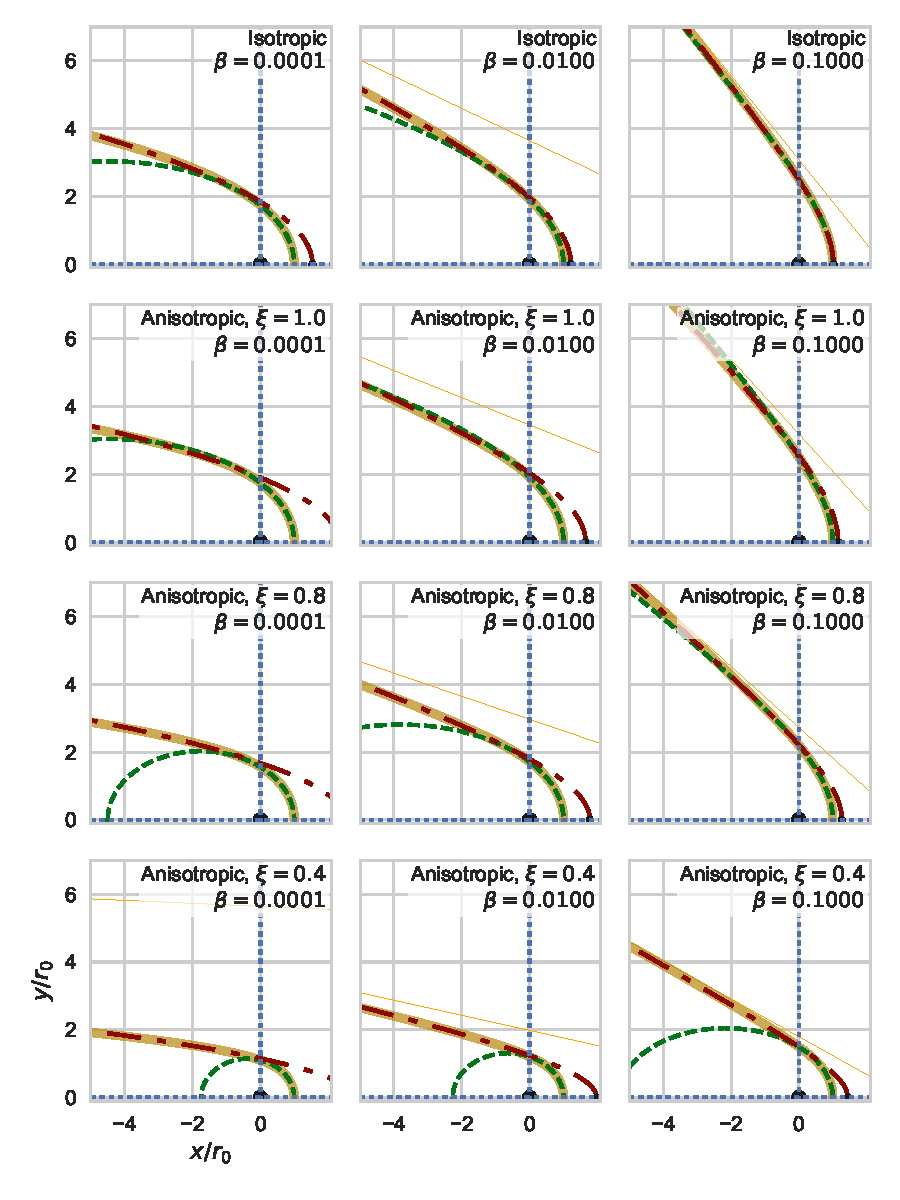
\includegraphics[width = 0.8\linewidth]{./Figures/conic-head-tail-analytic}
  \caption{Ajuste de dos cuádricas a las soluciones de capa delgada. La línea gruesa continua representa la forma de un choque bajo la aproximación de capa delgada (capítulo \ref{chap:hipersonica}) para los parámetros enlistados en cada pánel. La línea verde es el ajuste obtenido para la cabeza, mientras que la roja corresponde al ajuste para la cola.}
  \label{fig:conic-head-tail-fit}
\end{figure*}

En la figura \ref{fig:residuals} se muestra el residuo del ajuste en función del ańgulo polar, y observamos que para $\theta\sim 150^\circ$ el ajuste de la cola deja de ser bueno. Esto implica que existe una inclinación límite $i_{lim}$ más allá de la cual no podemos confiar en el modelo propuesto en este trabajo, y que calcularemos en la \S \ref{sec:proyection-CRW}.

\section{Ajustes a la cabeza}

Utilizando las ecuación (\ref{eq:thc2})  de la \S \ref{sec:conic-char-radii} y las ecuaciones (\ref{eq:CRW-Rc}) y (\ref{eq:CRW-R90}) de la \S \ref{sec:CRW-2-winds} podemos calcular el parámetro $\theta_c$ que nos indicará el tipo de cónica que ajusta mejor a cada solución del modelo de capa delgada
en función de los parámetros $\beta$ y $\xi$: 

 \begin{align}
   \tan\theta_c = \pm\left|\frac{3\xi\left(1 + \beta^{1/2}\right)^2}{\left(1 - \xi\beta\right)^2
   \left(1 + \frac{1}{5}\xi\beta\right)} - \frac{2}{\left|1 - 2\gamma\right|}\right|^{1/2}
 \end{align}

 En la figura  se ilustra la dependencia de $\theta_c$ con los parámetros $\beta$ y $\xi$, así como al tipo de cónica que ajusta mejor tanto la cabeza como la cola de cada solución a la forma de los choques de proa.
 
 \section{Ajustes a la cola}
\label{sec:tail-fit}
 En el caso general del problema de capa delgada, el comportamiento de la cola tiende a ser hiperbólico, dado que
 el ángulo polar $\theta$ tiende a un valor asintótico denominado como $\theta_\infty$. Este ángulo es tal que
 $\theta_\infty + \theta_{1\infty} = \pi$ y se calcula resolviendo la siguiente ecuación explícita:

 \begin{align}
   
 \end{align}

 El ajuste a la hipérbola se logra ajustando tres parámetros fundamentales: $\theta_c = \theta_\infty - \pi$, la distancia entre la hipérbola y el centro de ésta a lo largo del eje focal $a_t$ y la distancia entre el origen y el centro de la hipérbola $x_{0,t}$. $a_t$ y $x_{0,t}$ se obtienen inicialmente con un ajuste numérico para una malla de valores de $\beta$ y $\xi$. Posteriormente hacemos tres ajustes anidados en tres niveles para determinar de manera analítica los parámetros de la hipérbola en función de $\beta$ y $\xi$. A continuación mostramos las funciones y los parámetros que mejor ajustan a la cola para cada solución a la forma de los choques de proa. CAbe destacara

 \begin{align}
   x_{0,t} = 0.7\beta^{-0.55}\left[C_3\left(\log_{10}\beta\right)^3 + C_2\left(\log_{10}\beta\right)^2 +
   C_1\left(\log_{10}\beta\right) + C_0\right] \label{eq:tail-analytic-x0}\\
   (x_{0,t} - a_t) = D_2\left(\log_{10}\beta\right)^2 + D_1\left(\log_{10}\beta\right) + D_0
   \label{eq:tail-analytic-x0-minus-a}
 \end{align}

 Donde:
 
 \begin{alignat}{2}
   \label{eq:tail-analytic-coeffs-c}
   C_k &= c_{2,k}\xi^2 + c_{1,k}\xi + c_{0,k} & \mathrm{para~}k=[0,1,2,3] \\
   \label{eq:tail-analytic-coeffs-d}
   D_k &= d_{2,k}\xi^2 + d_{1,k}\xi + d_{0,k} & \mathrm{para~}k=[0,1,2]
 \end{alignat}

 Los coeficientes de los ajustes para la cola se muestran en la tabla \ref{tab:tail-fit-coeffs}:


\newcommand\iso{\ensuremath{^{\mathrm{iso}}}}

\begin{table}
  \caption{Coeficientes del ajuste hiperbólico a la cola de los choques de Proa}
  \label{tab:tail-fit-coeffs}
  \renewcommand\arraystretch{1.2}
  \setlength\tabcolsep{0.5\tabcolsep}
  \begin{tabular}{@{}llll@{}}
    \toprule
    Ecuación~(\ref{eq:tail-analytic-x0}) & 
    \multicolumn{3}{l}{
    Ecuación~(\ref{eq:tail-analytic-coeffs-c}) \dotfill
    } \\ \midrule
    \( C\iso_0 = +1.3195     \)    
    & \( c_{0,0} = +2.0758   \)  
    & \( c_{1,0} = -0.2309   \)  
    & \( c_{2,0} = -0.2532   \)\\
      \( C\iso_1 = +0.4229     \)    
    & \( c_{0,1} = +0.9571   \)  
    & \( c_{1,1} = -0.1530   \)  
    & \( c_{2,1} = -0.2487   \)\\
      \( C\iso_2 = +0.1092     \)    
    & \( c_{0,2} = +0.2528   \)  
    & \( c_{1,2} = -0.0360   \)  
    & \( c_{2,2} = -0.0794   \)\\
      \( C\iso_3 = +0.0051     \)    
    & \( c_{0,3} = +0.0171   \)  
    & \( c_{1,3} = -0.0010   \)  
    & \( c_{2,3} = -0.0095   \)\\ \midrule
    Ecuación~(\ref{eq:tail-analytic-x0-minus-a}) &
    \multicolumn{3}{l}{
    Ecuación~(\ref{eq:tail-analytic-coeffs-d}) \dotfill
    } \\ \midrule
    \( D\iso_0 = +0.7962   \)    
    & \( d_{0,0} = +0.8516 \)  
    & \( d_{1,0} = -0.0907 \)  
    & \( d_{2,0} = -0.2002 \)\\
      \( D\iso_1 = -0.2363   \)    
    & \( d_{0,1} = -0.7620 \)  
    & \( d_{1,1} = +0.1411 \)  
    & \( d_{2,1} = -0.0295 \)\\
      \( D\iso_2 = -0.0126   \)    
    & \( d_{0,2} = -0.0683 \)  
    & \( d_{1,2} = +0.0390 \)  
    & \( d_{2,2} = -0.0236 \)\\
    \bottomrule
  \end{tabular}
\end{table}

 
 En el apéndice \ref{app:tail-fit} se muestran los detalles de cómo se obtuvieron los coeficientes de la tabla \ref{tab:tail-fit-coeffs}. 
 
 \subsection{Ajustes a la cabeza y la cola en el caso de la interacción con un viento plano--paralelo}

 En este caso el ajuste a la cabeza es muy simple, utilizando los resultados para sus radios característicos (ecuaciones (\ref{eq:R90-Wilkin}) y (\ref{eq:Rc-Wilkin})) encontramos que el ajuste a la cabeza corresponde con una elipse tal que $\tan\theta_c = \frac{1}{3}$.
 Para el ajuste a la cola encontramos que ninguna de las cuádricas da una buena aproximación a la forma de la  cola, pero contamos con la forma explícita del choque de proa (ecuación (\ref{eq:R-Wilkin})) así que ningún ajuste fue necesario.
 
 \section{Proyección en el plano del cielo para el modelo de capa delgada}
\label{sec:proyection-CRW}
 La proyección en el plano del cielo se realizó utilizando las ecuaciones (\ref{eq:Rpc-quad}), (\ref{eq:thcp-quad}) y (\ref{eq:Rp90-quad}) para los ajuste de la cabeza y de la cola, respectivamente.

 En la figura \ref{fig:residuals} se muestra el residuo del ajuste de diferentes soluciones contra el ángulo polar $\theta$. Se puede apreciar que para cierto valor de $\theta$, que podemos denominar como $\theta_{tran}$, ocurre la transición donde el mejor ajuste deja de ser el de la cabeza y el ajuste de la cola empieza a ser más efectivo. Debido a esto, tenemos que tener cuidado qué ajuste elegir para calcular los radios característicos aparentes. Si $\theta_0 < \theta_{tran}$ entonces podemos utilizar el ajuste a la cabeza para calcular el radio de curvatura aparente, en caso contrario se tiene que utilizar el ajuste a la cola, lo que ocurre a inclinaciones altas. Para calcular $R'_{90}$ hay que vigilar si $\theta_{90}$ es mayor o menor a $\theta_{tran}$ para decidir qué ajuste utilizar. En este último caso será el de la cola para la mayoría de las inclinaciones.

 \begin{figure}
   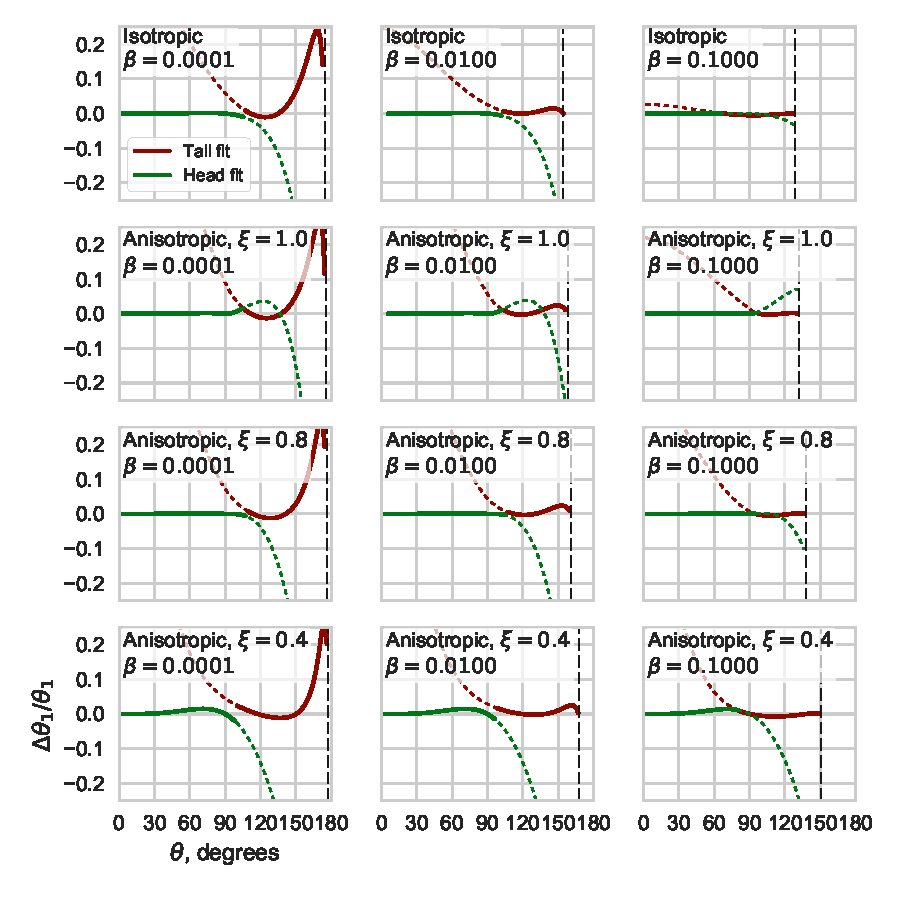
\includegraphics[width=0.5\linewidth]{./Figures/conic-head-tail-residuals}
   \caption{Residuo del ajuste de las cónicas a la forma del choque. La línea verde muestra el residuo del ajuste a la cabeza y la roja el ajuste a la cola. En todos los casos existe un valor de $\theta_{tran}$ donde para $\theta < \theta_{tran}$ el mejor ajuste es el de la cabeza y para $\theta \geq \theta_{tran}$ el mejor ajuste es el de la cola}.
   \label{fig:residuals}
 \end{figure}

 Utilizando las ecuaciones (\ref{eq:t-th-conversion}), (\ref{eq:t0}) y (\ref{eq:t90}) calculamos los valores para $\theta_0$ y $\theta_{90}$ para las cuádricas:
 \begin{align}
   \cot\theta_0 = \cot\theta_c\cot{i} + \frac{x_0}{b} \sqrt{\cot^2\theta_c\cot^2{i}\pm 1}
 \end{align}

 Utilizando las ecuaciones (\ref{eq:x0}), (\ref{eq:til-b}) y (\ref{eq:thc2}) encontramos que:

 \begin{align}
   \frac{x_0}{b} = \frac{|\tan\theta_c|}{\tilde{R}_c} - |\cot\theta_c|
 \end{align}

 Por otro lado:

 \begin{align}
   \Cot(\theta_{90}) = f_2(i;\theta_c)\left[\frac{x_0}{b} - \frac{x_0}{a}\frac{|\cot \theta_c|}{f^2(i;\theta_c)}\right] 
 \end{align}

 Donde $f(i;\theta_c)$ fue definido en la sección \ref{sec:quadrics} y:
 \begin{align}
   f_2(i;\theta_c)\equiv\left(1 \mp \frac{x^2_0}{a^2f^4(i;\theta_c)}\right)^{-1/2}
 \end{align}

 









 